\begin{multicols}{2}
  \section{Determine si las siguientes integrales convergen o divergen:}

  \begin{enumerate}
    \item
    \[
      \displaystyle \int_{3}^{7} \frac{2}{x-3} \, dx
    \]
  La función \( f(x) = \frac{2}{x-3} \) tiene una discontinuidad en \( x = 3 \) que además se encuentra dentro de los límites de initegración. Por lo tanto, esta es una integral impropia.
  \[
    \int_{3}^{7} \frac{2}{x-3} \, dx = 2 \lim_{a \to 3^{+}} \int_{a}^{7} \frac{1}{x-3} \, dx 
  \]
  Hallando la antiderivada:
  \[
    \int \frac{1}{x-3} \, dx = \ln{|
    x-3|} + C
  \]
  Luego, 
  \[
    \begin{aligned}
      2 \lim_{a \to 3^{+}} \int_{a}^{7} \frac{1}{x-3} \, dx &= 2 \lim_{a \to 3^{+}} \left[ \ln{|x-3|} \right]_{a}^{7} \\
      &= 2 \lim_{a \to 3^{+}} \left[ \ln{|4|} - \ln{|x-3|} \right]_{a}^{7} \\
      &= 2 \left(\ln{4} - \lim_{a \to 3^{+}} \ln{|a-3|}\right)
    \end{aligned}
  \]
  Considerando:
  \begin{center}
    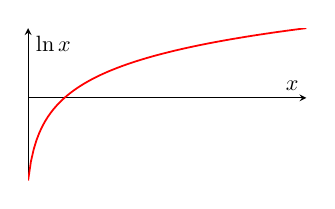
\begin{tikzpicture}[scale=0.8]
      \begin{axis}[
        axis lines = middle,
        xlabel = $x$,
          ylabel = {$\ln x$},
          domain=0.1:7,
          samples=100,
          width=6cm,
          height=4cm,
          xtick=\empty,
          ytick=\empty,
          grid=none,
              ]
          \addplot[red, thick] {ln(x)};
      \end{axis}
    \end{tikzpicture}
  \end{center}
  Por lo tanto,
  \[
    \begin{aligned}
      2 \left(\ln{4} - \lim_{a \to 3^{+}} \ln{|a-3|}\right) &= 2 (\ln{4} - (-\infty)) \\
      &= 2 (\ln{4} + \infty) = \infty
    \end{aligned}
  \]
  Por lo tanto, la integral diverge.  
  
    \item
    \[
      \displaystyle \int_{0}^{1} \frac{3}{x^{2}+x-2} \, dx
    \]
    Tratando algebraicamente:
    \[\begin{aligned}
      x^{2}+x-2 &= (x+2)(x-1) \\
      \frac{3}{x^{2}+x-2} &= \frac{3}{(x+2)(x-1)} \\
      &= \frac{A}{x+2} + \frac{B}{x-1} \\
      3 &= A(x-1) + B(x+2) \\
      3 &= (A+B)x + (-A+2B)
    \end{aligned}
    \]
    De aquí se concluye:
    \[
    \begin{cases}
    A + B = 0 \\
    - A + 2B = 3
    \end{cases} \implies 
    \begin{cases}
    A = -1 \\
    B = 1
    \end{cases}
    \]
    Entonces se tiene:
    \[\begin{aligned}
      \int_{0}^{1} \frac{3}{x^{2}+x-2} \, dx &= \int_{0}^{1} \left( \frac{-1}{x+2} + \frac{1}{x-1} \right) \, dx \\  
      &= \int_{0}^{1} \frac{1}{x-1} \, dx - \int_{0}^{1} \frac{1}{x+2} \, dx
      \end{aligned}
    \]
    De la integral, se tiene que la función que se integra tiene discontinuidad en \( x = 1 \) y en \( x = -2 \). Sin embargo, solo la discontinuidad en \( x = 1 \) se encuentra dentro de los límites de integración. Por lo tanto, esta es una integral impropia.
    \[
    \begin{aligned}
    &\int_{0}^{1} \frac{1}{x-1} \, dx - \int_{0}^{1} \frac{1}{x+2} \, dx \\
    &= \lim_{b \to 1^{-}} \int_{0}^{b} \frac{1}{x-1} \, dx - \int_{0}^{1} \frac{1}{x+2} \, dx
    \end{aligned}
    \]
    Hallando las antiderivadas:
    \begin{itemize}
      \item \[
        \int \frac{1}{x-1} \, dx = \ln{|x-1|} + C
      \]
      \item \[
        \int \frac{1}{x+2} \, dx = \ln{|x+2|} + C
      \]
    \end{itemize}
    Luego,
    \[
      \begin{aligned}
        &\lim_{b \to 1^{-}} \int_{0}^{b} \frac{1}{x-1} \, dx - \int_{0}^{1} \frac{1}{x+2} \, dx \\
        &= \lim_{b \to 1^{-}} \left[ \ln{|x-1|} \right]_{0}^{b} - \left[ \ln{|x+2|} \right]_{0}^{1} \\
        &= \lim_{b \to 1^{-}} \left( \ln{|b-1|}\right) - \ln{1} - \ln{3} + \ln{2} \\
        &= -\infty - 0 - \ln{3} + \ln{2} = -\infty
      \end{aligned}
    \]
    Por lo tanto, la integral diverge.
    \item
    \[
      \displaystyle \int_{-\infty}^{\infty} 3|x|e^{-x^{2}} \, dx
    \]
    Por la definición de valor absoluto, se tiene:
    \[
      |x| =
      \begin{cases}
        x, & x \geq 0 \\
        -x, & x < 0
      \end{cases}
    \]
    Entonces,
    \[
      \begin{aligned}
        &\int_{-\infty}^{\infty} 3|x|e^{-x^{2}} \, dx \\
        &= 3\left(\int_{0}^{\infty} xe^{-x^{2}} \, dx - \int_{-\infty}^{0} xe^{-x^{2}} \, dx\right)
      \end{aligned}
    \]
    Considerando que en los límites de integración hay infinito, esta es una integral impropia. Entonces,
    \[
      \begin{aligned}
        &3\left(\int_{0}^{\infty} xe^{-x^{2}} \, dx - \int_{-\infty}^{0} xe^{-x^{2}} \, dx\right) \\
        &= 3\left(\lim_{b \to \infty^{-}} \int_{0}^{b} xe^{-x^{2}} \, dx - \lim_{a \to -\infty^{+}} \int_{a}^{0} xe^{-x^{2}} \, dx\right)
      \end{aligned}
    \]
    Consideremos el cambio de variable,
    \[
      u = x^{2} \implies du = 2x \, dx \implies \frac{1}{2} du = x \, dx
    \]
    Luego,
    \[
      \begin{aligned}
        &3\left(\lim_{b \to \infty^{-}} \int_{0}^{b} xe^{-x^{2}} \, dx - \lim_{a \to \infty^{+}} \int_{a}^{0} xe^{-x^{2}} \, dx\right) \\
        &= 3\left(\lim_{b \to \infty^{-}} \int_{0}^{b} \frac{1}{2} e^{-u} \, du - \lim_{a \to \infty^{+}} \int_{a}^{0} \frac{1}{2} e^{-u} \, du\right) \\
        &= \frac{3}{2}\left(\lim_{b \to \infty^{-}} \int_{0}^{b} e^{-u} \, du - \lim_{a \to \infty^{+}} \int_{a}^{0} e^{-u} \, du\right)
      \end{aligned}
    \]
    \textbf{Obs:}\textit{\quad Se consideró también el cambio en los límites de integración.}

    Calculando las antiderivadas:
    \[
      \int e^{-u} \, du = -e^{-u} + C
    \]
    Entonces,
    \[
      \begin{aligned}
        &\frac{3}{2}\left(\lim_{b \to \infty^{-}} \int_{0}^{b} e^{-u} \, du - \lim_{a \to \infty^{+}} \int_{a}^{0} e^{-u} \, du\right) \\
        &= \frac{3}{2}\left(\lim_{b \to \infty^{-}} \left[-e^{-u}\right]_{0}^{b} - \lim_{a \to \infty^{+}} \left[-e^{-u}\right]_{a}^{0}\right) \\
        &= \frac{3}{2}\left(\lim_{b \to \infty^{-}} (-e^{-b} + 1) - \lim_{a \to \infty^{+}} (-1 + e^{-a})\right) \\
        &= \frac{3}{2}\left((0 + 1) - (-1 + 0)\right) = \frac{3}{2}(1 + 1) = 3
      \end{aligned}
    \]
    Por lo tanto, la integral converge y su valor es \( 3 \).
\end{enumerate}
\section{Usando la definición de función Gamma, evalúe las siguientes integrales:}
Función Gamma:
\begin{center}
  \fbox{
    \(
      \Gamma(n) = \int_{0}^{\infty} x^{n-1} e^{-x} \, dx
    \)
  }
\end{center}
\begin{enumerate}
  \item \[
    \displaystyle \int_{0}^{\infty} e^{-10x}\sqrt{x^{5}} \, dx
  \]
  Considerando el cambio de variable,
  \[
    u = 10x \implies du = 10 \, dx \implies dx = \frac{1}{10} du
  \]
  Entonces,
  \[
    \begin{aligned}
      \int_{0}^{\infty} e^{-10x}\sqrt{x^{5}} \, dx &= \int_{0}^{\infty} e^{-u} \left(\frac{u}{10}\right)^{\frac{5}{2}} \frac{1}{10} \, du \\
      &= \int_{0}^{\infty} e^{-u} \frac{u^{\frac{5}{2}}}{10^{\frac{5}{2}}} \cdot \frac{1}{10} \, du \\
      &= \frac{1}{\sqrt{10^{7}}} \int_{0}^{\infty} e^{-u} u^{\frac{5}{2}} \, du
    \end{aligned}
  \]
  Por la definición de función Gamma, se tiene:
  \[
    \Gamma\left(\frac{7}{2}\right) = \int_{0}^{\infty} e^{-u} u^{\frac{7}{2}-1} \,du
  \]
  Entonces,
  \[
    \int_{0}^{\infty} e^{-10x}\sqrt{x^{5}} \, dx = \frac{1}{\sqrt{10^{7}}} \Gamma\left(\frac{7}{2}\right)
  \]
  De acuerdo con la propiedad de la función Gamma:
  \[
    \frac{1}{\sqrt{10^{7}}} \Gamma\left(\frac{7}{2}\right) = \frac{1}{\sqrt{10^{7}}} \cdot \frac{5}{2} \cdot \frac{3}{2} \cdot \frac{1}{2} \cdot \sqrt{\pi} = \frac{15\sqrt{\pi}}{8\sqrt{10^{7}}}
  \]
  \item \[
    \displaystyle \int_{0}^{\infty} \dfrac{\sqrt{x^{9}}}{e^{3x}} \, dx
  \]
  Reescribiendo la integral:
  \[
    \int_{0}^{\infty} \dfrac{\sqrt{x^{9}}}{e^{3x}} \, dx = \int_{0}^{\infty} e^{-3x} x^{\frac{9}{2}} \, dx
  \]
  Considerando el cambio de variable,
  \[
    u = 3x \implies du = 3 \, dx \implies dx = \frac{1}{3} du
  \]
  Entonces,
  \[
    \begin{aligned}
      \int_{0}^{\infty} e^{-3x} x^{\frac{9}{2}} \, dx &= \int_{0}^{\infty} e^{-u} \left(\frac{u}{3}\right)^{\frac{9}{2}} \frac{1}{3} \, du \\
      &= \int_{0}^{\infty} e^{-u} \frac{u^{\frac{9}{2}}}{3^{\frac{9}{2}}} \cdot \frac{1}{3} \, du \\
      &= \frac{1}{\sqrt{3^{11}}} \int_{0}^{\infty} e^{-u} u^{\frac{9}{2}} \, du
    \end{aligned}
  \]
  Por la definición de función Gamma, se tiene: 
  \[
    \Gamma\left(\frac{11}{2}\right) = \int_{0}^{\infty} e^{-u} u^{\frac{11}{2}-1} \,du
  \]
  Entonces,
  \[
    \int_{0}^{\infty} \dfrac{\sqrt{x^{9}}}{e^{3x}} \, dx = \frac{1}{\sqrt{3^{11}}} \Gamma\left(\frac{11}{2}\right)
  \]
  De acuerdo con la propiedad de la función Gamma:
  \[
    \frac{1}{\sqrt{3^{11}}} \Gamma\left(\frac{11}{2}\right) = \frac{1}{\sqrt{3^{11}}} \cdot \frac{9}{2} \cdot \frac{7}{2} \cdot \frac{5}{2} \cdot \frac{3}{2} \cdot \frac{1}{2} \cdot \sqrt{\pi} = \frac{945\sqrt{\pi}}{32\sqrt{3^{11}}}
  \]
\end{enumerate}
\section{Usando la definición de función Beta, evalúe las siguientes integrales:}
Función Beta:
\begin{center}
  \fbox{
    \(
      B(m,n) = \int_{0}^{1} x^{m-1} (1-x)^{n-1} \, dx
    \)
  }
\end{center}
\begin{enumerate}
  \item \[
    \displaystyle \int_{0}^{5} \dfrac{x^{3}}{\sqrt{5-x}} \, dx
  \]
  Considerando el intervalo de integración:
  \[
    0 \leq x \leq 5 \implies 0 \leq \frac{x}{5} \leq 1
  \]
  Con ello el cambio de variable:
  \[
    \begin{aligned}
      u &= \frac{x}{5} \implies x = 5u \\
      dx &= 5 \, du
    \end{aligned}
  \]
  Entonces,
  \[
    \begin{aligned}
      \int_{0}^{5} \dfrac{x^{3}}{\sqrt{5-x}} \, dx &= \int_{0}^{1} \dfrac{(5u)^{3}}{\sqrt{5-5u}} \cdot 5 \, du \\
      &= 125 \sqrt{5} \int_{0}^{1} \dfrac{u^{3}}{\sqrt{1-u}} \, du \\
      &= 125 \sqrt{5} \int_{0}^{1} u^{3} (1-u)^{-\frac{1}{2}} \, du
    \end{aligned}
  \]
  Por la definición de función Beta, se tiene:
  \[
    B(4, \tfrac{1}{2}) = \int_{0}^{1} u^{4-1} (1-u)^{\frac{1}{2}-1} \, du
  \]
  Según la propiedad de la función Beta:
  \[
    B(m,n) = \frac{\Gamma(m)\Gamma(n)}{\Gamma(m+n)}
  \]
  Entonces,
  \[
    \int_{0}^{5} \dfrac{x^{3}}{\sqrt{5-x}} \, dx = 125 \sqrt{5} B(4, \tfrac{1}{2}) = 125 \sqrt{5} \cdot \frac{\Gamma(4)\Gamma(\tfrac{1}{2})}{\Gamma(\tfrac{9}{2})}
  \]
  Por lo tanto,
  \[
    \begin{aligned}
      125 \sqrt{5} \cdot \frac{\Gamma(4)\Gamma(\tfrac{1}{2})}{\Gamma(\tfrac{9}{2})} &= 125 \sqrt{5} \cdot \frac{3!}{\frac{7}{2} \cdot \frac{5}{2} \cdot \frac{3}{2} \cdot \frac{1}{2}}
    \end{aligned}
  \]
  \columnbreak
  \item \[
    \displaystyle \int_{0}^{6} \dfrac{x^{4}}{\sqrt{6-x}} \, dx
  \]
  Considerando el intervalo de integración:
  \[
    0 \leq x \leq 6 \implies 0 \leq \frac{x}{6} \leq 1
  \]
  Con ello el cambio de variable:
  \[
    \begin{aligned}
      u &= \frac{x}{6} \implies x = 6u \\
      dx &= 6 \, du
    \end{aligned}
  \]
  Entonces,
  \[
    \begin{aligned}
      \int_{0}^{6} \dfrac{x^{4}}{\sqrt{6-x}} \, dx &= \int_{0}^{1} \dfrac{(6u)^{4}}{\sqrt{6-6u}} \cdot 6 \, du \\
      &= 6^{3} \sqrt{6} \int_{0}^{1} \dfrac{u^{4}}{\sqrt{1-u}} \, du \\
      &= 6^{3} \sqrt{6} \int_{0}^{1} u^{4} (1-u)^{-\frac{1}{2}} \, du
    \end{aligned}
  \]
  Por la definición de función Beta, se tiene:
  \[
    B(5, \tfrac{1}{2}) = \int_{0}^{1} u^{5-1} (1-u)^{\frac{1}{2}-1} \, du
  \]
  Entonces,
  \[
    \int_{0}^{6} \dfrac{x^{4}}{\sqrt{6-x}} \, dx = 6^{3} \sqrt{6} B(5, \tfrac{1}{2}) = 6^{3} \sqrt{6} \cdot \frac{\Gamma(5)\Gamma(\tfrac{1}{2})}{\Gamma(\tfrac{11}{2})}
  \]
  Por lo tanto,
  \[
    \begin{aligned}
      6^{3} \sqrt{6} \cdot \frac{\Gamma(5)\Gamma(\tfrac{1}{2})}{\Gamma(\tfrac{11}{2})} &= 6^{3} \sqrt{6} \cdot \frac{4!}{\frac{9}{2} \cdot \frac{7}{2} \cdot \frac{5}{2} \cdot \frac{3}{2} \cdot \frac{1}{2}}
    \end{aligned}
  \]
  \end{enumerate}
\newpage
  \section{Dada las siguientes coordenadas cartesianas, determine sus coordenadas polares y grafíquelas 
  en el plano polar.}
  \begin{enumerate}
    \item \[
      \displaystyle \left(-3.5\sqrt{3};-3.5\right)
    \] 
    Graficando el punto en el plano cartesiano:
    \begin{center}
      \begin{tikzpicture}[scale=0.8]
        \begin{axis}[
          axis lines = middle,
          xlabel = $x$,
          ylabel = {$y$},
          xmin=-7, xmax=1,
          ymin=-7, ymax=1,
          xtick={0},
          extra x ticks={-3.5*sqrt(3)},
          extra x tick labels={$-3.5\sqrt{3}$},
          ytick={-3.5,0},
        ]
          \addplot[only marks] coordinates {(-3.5*sqrt(3),-3.5)};
        \end{axis}
      \end{tikzpicture}
    \end{center}
    Aprovechando el triángulo notable:
    \begin{center}
      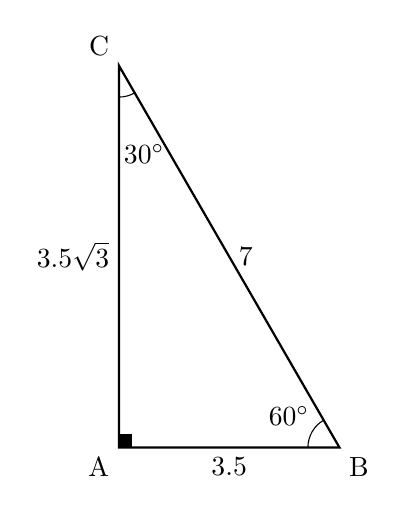
\begin{tikzpicture}[scale=0.8]
        % Draw triangle
        \draw[thick] (0,0) -- (3.5,0) -- (0,{3.5*sqrt(3)}) -- cycle;
        % Label vertices
        \node[below left] at (0,0) {A};
        \node[below right] at (3.5,0) {B};
        \node[above left] at (0,{3.5*sqrt(3)}) {C};
        % Label sides
        \node[below] at (1.75,0) {$3.5$};
        \node[left] at (0,{1.75*sqrt(3)}) {$3.5\sqrt{3}$};
        \node[right] at (1.75,{1.75*sqrt(3)}) {$7$};
        % Mark angles
        % Marca negra en el vértice A
        \filldraw[fill=black] (0,0) rectangle +(0.2,0.2);
        \draw (0,{3.5*sqrt(3)-0.5}) arc (270:300:0.5);
        \node at (0.4,{3.5*sqrt(3)-1.4}) {$30^\circ$};
        \draw ({3.5-0.5},0) arc (180:120:0.5);
        \node at (2.7,0.5) {$60^\circ$};
    \end{tikzpicture}
    \end{center}


    Por ser un triángulo rectángulo, se tiene:
    \[
      \tan{\theta} = \frac{-3.5}{-3.5\sqrt{3}} = \frac{1}{\sqrt{3}} \implies \theta = 30^\circ = \frac{\pi}{6}
    \]
    Considerando que el punto se encuentra en el tercer cuadrante, se tiene:
    \[
      \theta = 180^\circ + 30^\circ = 210^\circ = \frac{7\pi}{6}
    \]
    Dibujando en el plano polar,
    \begin{center}
      \begin{tikzpicture}
        \begin{polaraxis}[
            axis lines = middle,
            xtick={0,30,...,330},   % divisiones angulares
            xticklabels={,, , , , , , , , , ,},
            ytick={1,3,...,7},      % divisiones radiales
            ymin=0, ymax=7,
            extra x ticks={0,90,180,270},
            extra x tick labels={$$,,,$$},
            extra y ticks={0},
            extra y tick labels={},
          ]
          % punto en coordenadas polares (ángulo en grados, radio)
          \addplot[only marks, mark=*] coordinates {(210,7)};
          % Línea que une el centro con el punto (210°, 7)
          \draw[thick, black] (axis cs:0,0) -- (axis cs:210,7);
          % Etiqueta para indicar la coordenada del punto
          \node at (axis cs:210,7.2) [anchor=west] {$(7,\frac{7\pi}{6})$};
        \end{polaraxis}
      \end{tikzpicture}
    \end{center}
    \item \[
      \displaystyle \left(12;-12\right)
    \]
    Graficando el punto en el plano cartesiano:
    \begin{center}
      \begin{tikzpicture}[scale=0.8]
        \begin{axis}[
          axis lines = middle,
          xlabel = $x$,
          ylabel = {$y$},
          xmin=-1, xmax=13,
          ymin=-13, ymax=1,
          xtick={0,12},
          ytick={-12,0},
        ]
          \addplot[only marks] coordinates {(12,-12)};
        \end{axis}
      \end{tikzpicture}
    \end{center}
    Considerando el triángulo rectángulo:
    \begin{center}
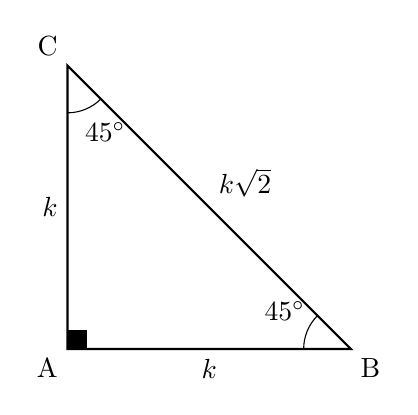
\begin{tikzpicture}[scale=1.2]
  % Triángulo rectángulo isósceles
  \draw[thick] (0,0) -- (3,0) -- (0,3) -- cycle;

  % Vértices
  \node[below left] at (0,0) {A};
  \node[below right] at (3,0) {B};
  \node[above left] at (0,3) {C};

  % Etiquetas de lados
  \node[below] at (1.5,0) {$k$};
  \node[left] at (0,1.5) {$k$};
  \node[above right] at (1.5,1.5) {$k\sqrt{2}$};

  % Ángulo recto en A
  \filldraw[fill=black] (0,0) rectangle +(0.2,0.2);

  % Arcos para ángulos de 45°
  \draw (2.5,0) arc (180:135:0.5);
  \node at (2.3,0.4) {$45^\circ$};

  \draw (0,2.5) arc (270:315:0.5);
  \node at (0.4,2.3) {$45^\circ$};
\end{tikzpicture}
\end{center}
    Por ser un triángulo rectángulo isósceles, se tiene:
    \[
      \tan{\theta} = \frac{-12}{12} = -1 \implies \theta = -45^\circ = -\frac{\pi}{4}
    \]
    Considerando que el punto se encuentra en el cuarto cuadrante, se tiene:
    \[
      \theta = 360^\circ - 45^\circ = 315^\circ = \frac{7\pi}{4}
    \]
    Dibujando en el plano polar,
    \begin{center}
      \begin{tikzpicture}
        \begin{polaraxis}[
            axis lines = middle,
            xtick={0,30,...,330},   % divisiones angulares
            xticklabels={,, , , , , , , , , ,},
            ytick={1,3,...,13},      % divisiones radiales
            ymin=0, ymax=13,
            extra x ticks={0,90,180,270},
            extra x tick labels={$$,,,$$},
            extra y ticks={0},
            extra y tick labels={},
          ]
          % punto en coordenadas polares (ángulo en grados, radio)
          \addplot[only marks, mark=*] coordinates {(315,12)};
          % Línea que une el centro con el punto (315°, 12)
          \draw[thick, black] (axis cs:0,0) -- (axis cs:315,12);
          % Etiqueta para indicar la coordenada del punto
          \node at (axis cs:315,12.2) [anchor=east] {$(12,\frac{7\pi}{4})$};
        \end{polaraxis}
      \end{tikzpicture}
    \end{center}
  \end{enumerate}
  \section{Determina la gráfica de las siguientes ecuaciones polares:}
  \begin{enumerate}
    \item \[
      r = 4-8\cos{\theta}
    \]
    Tabulando valores desde \( 0 \) hasta \( 2\pi \) con incrementos de \( \frac{\pi}{12} \):
    \begin{center}
      \begin{tabular}{|c|c||c|c|}
        \hline
        \( \theta \) & \( r \) & \( \theta \) & \( r \) \\
        \hline
        \( 0 \) & \( -4 \) & \( \frac{\pi}{12} \) & \( -2.071 \) \\
        \( \frac{\pi}{6} \) & \( 0 \) & \( \frac{\pi}{4} \) & \( 1.172 \) \\
        \( \frac{\pi}{3} \) & \( 2 \) & \( \frac{5\pi}{12} \) & \( 2.598 \) \\
        \( \frac{\pi}{2} \) & \( 4 \) & \( \frac{7\pi}{12} \) & \( 5.402 \) \\
        \( \frac{2\pi}{3} \) & \( 6 \) & \( \frac{3\pi}{4} \) & \( 6.828 \) \\
        \( \frac{5\pi}{6} \) & \( 8 \) & \( \frac{11\pi}{12} \) & \( 9.071 \) \\
        \( \pi \) & \( 12 \) & \( \frac{13\pi}{12} \) & \( 9.071 \) \\
        \( \frac{7\pi}{6} \) & \( 8 \) & \( \frac{5\pi}{4} \) & \( 6.828 \) \\
        \( \frac{4\pi}{3} \) & \( 6 \) & \( \frac{17\pi}{12} \) & \( 5.402 \) \\
        \( \frac{3\pi}{2} \) & \( 4 \) & \( \frac{19\pi}{12} \) & \( 2.598 \) \\
        \( \frac{11\pi}{6} \) & \( 2 \) & \( \frac{7\pi}{4} \) & \( 1.172 \) \\
        \( \frac{5\pi}{3} \) & \( 0 \) & \( \frac{19\pi}{12} \) & \( -2.071 \) \\
        \( \frac{3\pi}{2} \) & \( -4 \) & \( \frac{17\pi}{12} \) & \( -6.598 \) \\
        \( \frac{4\pi}{3} \) & \( -8 \) & \( \frac{5\pi}{4} \) & \( -9.656 \) \\
        \( \frac{7\pi}{6} \) & \( -12 \) & \( \frac{13\pi}{12} \) & \( -14.071 \) \\
        \hline
      \end{tabular}
    \end{center}
    Graficando en el plano polar:
    \begin{center}
      \begin{tikzpicture}
        \begin{polaraxis}[
            axis lines = middle,
            xtick={0,30,...,330},   % divisiones angulares
            xticklabels={,, , , , , , , , , ,},
            ytick={2,4,...,12},      % divisiones radiales
            ymin=0, ymax=12,
            extra x ticks={0,90,180,270},
            extra x tick labels={$$,,,$$},
            extra y ticks={0},
            extra y tick labels={},
          ]
          % punto en coordenadas polares (ángulo en grados, radio)
          \addplot[domain=0:360,samples=200,thick] {4 - 8*cos(x)};
        \end{polaraxis}
      \end{tikzpicture}
    \end{center}
    \item \[
      r = 2-5\sin{\theta}
    \]
    Tabulando valores desde \( 0 \) hasta \( 2\pi \) con incrementos de \( \frac{\pi}{12} \):
    \begin{center}
      \begin{tabular}{|c|c||c|c|}
        \hline
        \( \theta \) & \( r \) & \( \theta \) & \( r \) \\
        \hline
        \( 0 \) & \( 2 \) & \( \frac{\pi}{12} \) & \( -0.295 \) \\
        \( \frac{\pi}{6} \) & \( -0.5 \) & \( \frac{\pi}{4} \) & \( -1.536 \) \\
        \( \frac{\pi}{3} \) & \( -2.5 \) & \( \frac{5\pi}{12} \) & \( -3.536 \) \\
        \( \frac{\pi}{2} \) & \( -3 \) & \( \frac{7\pi}{12} \) & \( -1.964 \) \\
        \( \frac{2\pi}{3} \) & \( -1.5 \) & \( \frac{3\pi}{4} \) & \( -0.464 \) \\
        \( \frac{5\pi}{6} \) & \( 0.5 \) & \( \frac{11\pi}{12} \) & \( 1.705 \) \\
        \( \pi \) & \( 2 \) & \( \frac{13\pi}{12} \) & \( 1.705 \) \\
        \( \frac{7\pi}{6} \) & \( 0.5 \) & \( \frac{5\pi}{4} \) & \( -0.464 \) \\
        \( \frac{4\pi}{3} \) & \( -1.5 \) & \( \frac{17\pi}{12} \) & \( -1.964 \) \\
        \( \frac{3\pi}{2} \) & \( -3 \) & \( \frac{19\pi}{12} \) & \( -3.536 \) \\
        \( \frac{11\pi}{6} \) & \( -2.5 \) & \( \frac{7\pi}{4} \) & \( -1.536 \) \\
        \( \frac{5\pi}{3} \) & \( -0.5 \) & \( \frac{19\pi}{12} \) & \( -0.295 \) \\
        \( \frac{3\pi}{2} \) & \( 2 \) & & \\
        \hline
      \end{tabular}
    \end{center}
    Graficando en el plano polar:
    \begin{center}
      \begin{tikzpicture}
        \begin{polaraxis}[
            axis lines = middle,
            xtick={0,30,...,330},   % divisiones angulares
            xticklabels={,, , , , , , , , , ,},
            ytick={2,4,...,8},      % divisiones radiales
            ymin=0, ymax=8,
            extra x ticks={0,90,180,270},
            extra x tick labels={$$,,,$$},
            extra y ticks={0},
            extra y tick labels={},
          ]
          % punto en coordenadas polares (ángulo en grados, radio)
          \addplot[domain=0:360,samples=200,thick] {2 - 5*sin(x)};
        \end{polaraxis}
      \end{tikzpicture}
    \end{center}



\end{enumerate}
\end{multicols}